% !TEX program = xelatex
% vim:foldmethod=marker:foldmarker=<<<,>>>
\documentclass[compress]{beamer}

%<<< Preamble
\usepackage[english]{babel}
\usepackage{metalogo}
\usepackage{listings}
\usepackage{fontspec}
\usepackage{amsmath, amssymb}
\usepackage{stackrel}
\usepackage{tikz}
\usepackage{svg}
\usepackage{unicode-math}
\usepackage{subcaption}
\usepackage[theme=nord,charsperline=60,linenumbers]{jlcode}

\usetheme{Nord}

\setmainfont{Roboto}
% \setsansfont{DejaVu Serif}
% \setmonofont{CaskaydiaCove Nerd Font Mono}
\setmonofont{JuliaMono}


\makeatletter
\def\verbatim@nolig@list{}
\newcommand\pin{%
\parbox[t]{10pt}{\raisebox{0.2pt}{\usebeamercolor[fg]{mybullet}{$\ast$}}}}
\makeatother

\newcommand{\E}[1]{\ensuremath{E\left\{#1\right\}}}
\newcommand{\norm}[1]{\ensuremath{\lVert#1\rVert}}
\newcommand*{\thead}[1]{\multicolumn{1}{c}{\bfseries #1}}

\newfontfamily\tabulartext[SizeFeatures={Size=6}]{Roboto}

\hypersetup{
    colorlinks=true,
    urlcolor=NordBlue
}

\DeclareMathOperator*{\argmax}{argmax}
\DeclareMathOperator*{\Var}{Var}

\AtBeginDocument{
    \fontsize{8}{12}
    \selectfont

}

\AtBeginSection[]
{
    \begin{frame}[c,noframenumbering,plain]
        \tableofcontents[sectionstyle=show/hide,subsectionstyle=show/show/hide]
    \end{frame}
}


\AtBeginSubsection[]
{
    \begin{frame}[c,noframenumbering,plain]
        \tableofcontents[sectionstyle=show/hide,subsectionstyle=show/shaded/hide]
    \end{frame}
}
%>>>

\title{Project IV: Detection theory}
\subtitle{}
\author{\Large Simon Andreas Bjørn}
\date{\large March 14, 2023}

\begin{document}

\begin{frame}[plain,noframenumbering]
    \maketitle
\end{frame}

\begin{frame} % <<< PDF of measurement
    \frametitle{PDF of measurement}
    We first want to define the PDF of $f_\theta\left(x\right)$ which is the
    PDF of the {\em signal} + {\em noise}
    \begin{columns}
        \begin{column}{0.5\textwidth}
            We have a SNR-PDF model as shown on the right.
            We notice that:
            \begin{itemize}
                \item Noise PDF is i.i.d. and sampled around 0
                \item Signal PDF $f_\theta$ average at $\theta$
                \item The noise is additive to the signal
            \end{itemize}
        \end{column}
        \begin{column}{0.5\textwidth}
            \begin{figure}
                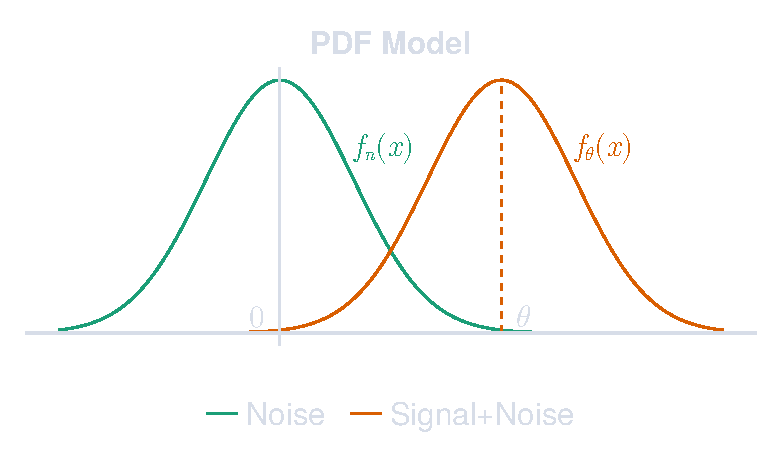
\includegraphics[width=\columnwidth]{"../PDFs.pdf"}
            \end{figure}
        \end{column}
    \end{columns}
    With the noise characterized and distributed $n \sim \mathcal{N}\left(0,\sigma\right)$, we have that
    the signal is distributed $s \sim \mathcal{N}\left(\theta,\sigma\right)$
    which gives the PDF
    \begin{equation*}
        f_\theta (x) = \frac{1}{\sqrt{2\pi}\sigma^2}e^{-\frac{\left(x-\theta\right)^2}{2\sigma^2}}
    \end{equation*}
\end{frame} % >>>

\begin{frame}[fragile] % <<< Specific detection problem
    \frametitle{Specific detection problem}
    Now we assume that $\theta = 5$ and $\sigma = 5$. Plotting this yields the 
    following plot
    \begin{columns}
        \begin{column}{0.5\textwidth}
            \begin{jllisting}[gobble=16]
                # Code for calculation
                θ = σ = 5
                fn = Normal(0,σ); fs = Normal(θ,σ)
                lines!(fn); lines!(fs)
            \end{jllisting}
        \end{column}
        \begin{column}{0.5\textwidth}
            \begin{figure}
                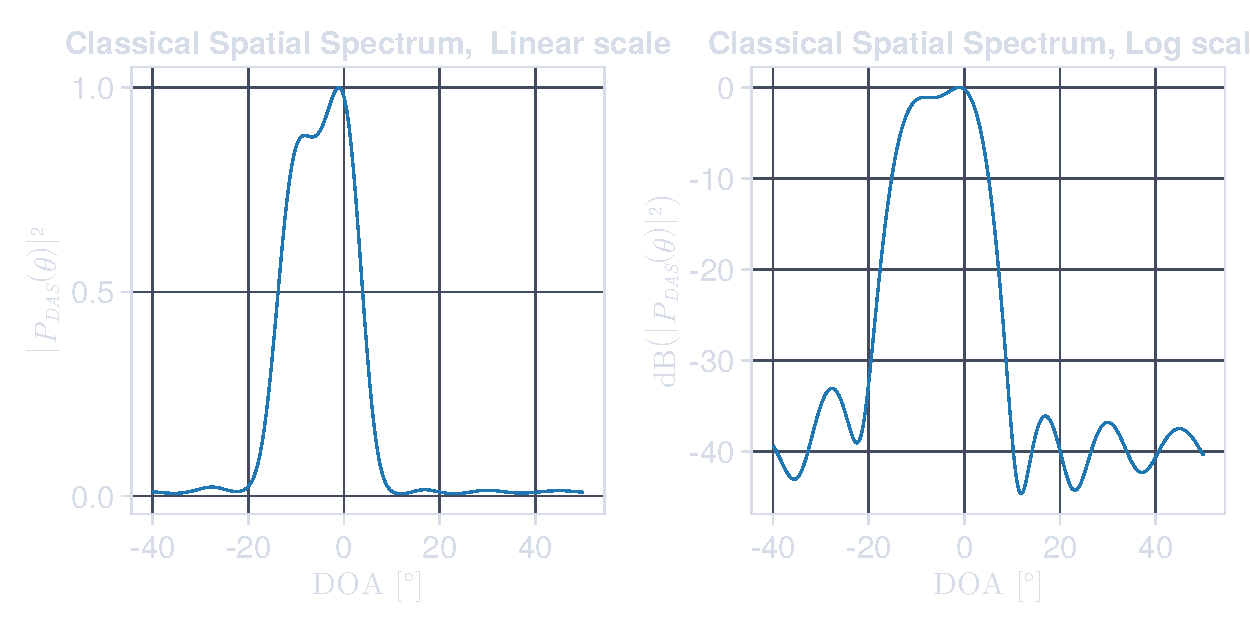
\includegraphics[width=\columnwidth]{"../b.pdf"}
            \end{figure}
        \end{column}
    \end{columns}
    I would say that this detection problem is quite tricky, because the two
    distributions are quite close together. The overlap of the false alarm and
    the detected signal is large, and so actually classifying what is noise
    and what is a true signal is difficult.
\end{frame} 
% >>>

\begin{frame}[fragile] % <<< CFAR detector with $P_{FA}] = 0.1$
    \frametitle{CFAR detector with $P_{FA} = 0.1$}
    
    We want a threshold $\beta$ such that $P_{FA} = 0.1$, which is given by 
    $$\int^{\infty}_{\beta}{f_n(x)dx} = P_n(\beta \le x) = 1-F_n(\beta)$$ where $F_n(x)$ is the CDF
    of the noise PDF. We know that the quantile function 
    $Q: \left[0,1\right] \rightarrow \mathbb{R}$ is defined as the inverse CDF, s.t.
    $Q_n(q) = F^{-1}_n(q)$. This gives the threshold 
    $\beta = Q_n\left(1-P_{FA}\right)$. With $\beta$ given, we can easly find $P_D$ by
    $1-F_s\left(\beta\right)$.

    \begin{columns}
        \begin{column}{0.5\textwidth}
            \begin{jllisting}[gobble=16]
                β = cquantile(fn, 0.1)
                P_fa = ccdf(fn, β)
                P_d  = ccdf(fs, β)
            \end{jllisting}

            As we can see in the plot and evaluations, we we get a threshold at
            $\beta = 6.41$ with a $P_D = 0.39$. That is, there is a 39\% chance
            for a detection.
        \end{column}
        \begin{column}{0.5\textwidth}
            \begin{figure}
                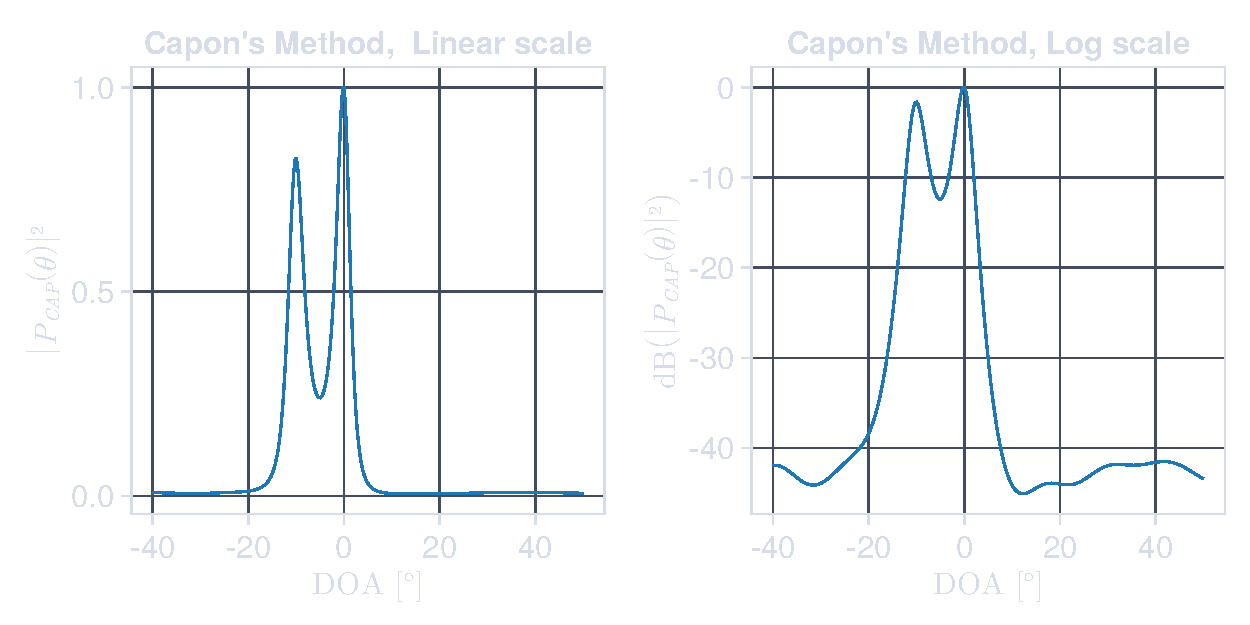
\includegraphics[width=\columnwidth]{"../c.pdf"}
            \end{figure}
        \end{column}
    \end{columns}
\end{frame}
% >>>

\end{document}
